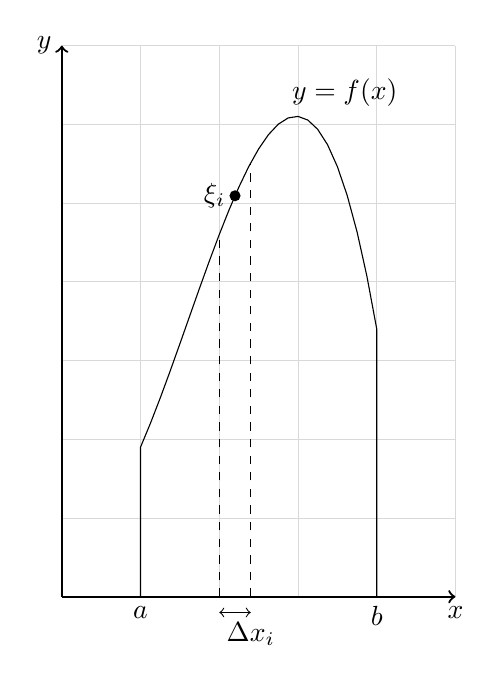
\begin{tikzpicture}
  \draw[very thin, gray!30, step = 1cm] (0, 0) grid (5, 7);
  \draw[domain = 1 : 4, variable = \x]
    (1, 0)
    -- plot ({\x}, {-0.5 * \x * \x * \x + 2.4 * \x * \x - \x + 1})
    -- (4, 0)
    -- cycle;

  \draw[<->] (2, -0.2) -- (2.4, -0.2) node [below] {\(\Delta x_{i}\)};
  \draw[dashed] (2, 0) -- (2, 4.6);
  \draw[dashed] (2.4, 0) -- (2.4, 5.512);
  \draw node[above, left] at (2.2, 5.092) {\(\xi_{i}\)};
  \fill[black] (2.2, 5.092) circle (2pt);

  \draw[thick] [->] (0, 0) -- (5, 0) node[right, below] {\(x\)};
  \draw[thick] [->] (0, 0) -- (0, 7) node[above, left] {\(y\)};
  \draw node[right] at (2.8, 6.4) {\(y = f(x)\)};
  \draw node[below] at (1, 0) {\(a\)};
  \draw node[below] at (4, 0) {\(b\)};
\end{tikzpicture}
